% TalentMatch — Project Specification (Cahier des Charges), presentation edition
% Build: xelatex TalentMatch_Cahier_des_Charges.tex  (run twice for the contents)
\documentclass[11pt,a4paper]{article}
\usepackage[a4paper,left=2.5cm,right=2.5cm,top=2.6cm,bottom=2.4cm]{geometry}
\usepackage{fontspec}
\setmainfont{Latin Modern Roman}
\setsansfont{Carlito}
\usepackage{xcolor}
\definecolor{accent}{HTML}{D9611A}
\definecolor{peach}{HTML}{FDF1E8}
\definecolor{grayline}{HTML}{BBBBBB}
\definecolor{graytext}{HTML}{777777}
\definecolor{graybox}{HTML}{F3F3F3}
\usepackage{graphicx}
\usepackage{booktabs,tabularx,xltabular,array}
\usepackage{enumitem}
\usepackage{needspace}
\usepackage{titlesec}
\usepackage[titles]{tocloft}
\usepackage{fancyhdr}
\usepackage[most]{tcolorbox}
\usepackage[hidelinks]{hyperref}
\usepackage{microtype}
\setlength{\parindent}{1.2em}
\setlength{\parskip}{0.2em}
\linespread{1.08}
\setlist{itemsep=1pt,topsep=3pt}

% ---------- Section style (Roman numerals, orange) ----------
\renewcommand{\thesection}{\Roman{section}}
\renewcommand{\thesubsection}{\arabic{section}.\arabic{subsection}}
\titleformat{\section}
  {\sffamily\bfseries\Large}{\textcolor{accent}{\thesection}\hspace{0.9em}}{0pt}{}[\vspace{-0.4em}{\color{grayline}\titlerule}]
\titlespacing*{\section}{0pt}{1.6em}{0.9em}
\titleformat{\subsection}
  {\sffamily\bfseries\normalsize}{\textcolor{accent}{\thesubsection}\hspace{0.7em}}{0pt}{}
\titlespacing*{\subsection}{0pt}{1.1em}{0.4em}

% ---------- Table of contents ----------
\renewcommand{\cftdot}{.}
\renewcommand{\cftdotsep}{2}
\renewcommand{\cftsecfont}{\sffamily\bfseries}
\renewcommand{\cftsecpagefont}{\sffamily\bfseries}
\renewcommand{\cftsubsecfont}{\color{graytext}\small}
\renewcommand{\cftsubsecpagefont}{\color{graytext}\small}
\renewcommand{\cftsecleader}{\cftdotfill{\cftdotsep}}
\setlength{\cftbeforesecskip}{0.55em}
\setlength{\cftbeforesubsecskip}{0.1em}
\setlength{\cftsecindent}{0pt}
\setlength{\cftsecnumwidth}{2.4em}
\setlength{\cftsubsecindent}{2.4em}
\setlength{\cftsubsecnumwidth}{2.4em}
\renewcommand{\cftsecpresnum}{\color{accent}}
\renewcommand{\cftsecaftersnum}{\color{black}}
\renewcommand{\cfttoctitlefont}{\sffamily\bfseries\Large}
\renewcommand{\cftaftertoctitle}{\par\vspace{-0.2em}{\color{accent}\rule{4cm}{0.8pt}}}

% ---------- Header / footer ----------
\pagestyle{fancy}
\fancyhf{}
\renewcommand{\headrulewidth}{0.3pt}
\renewcommand{\headrule}{\hbox to\headwidth{\color{grayline}\leaders\hrule height \headrulewidth\hfill}}
\fancyhead[L]{\sffamily\footnotesize\color{graytext} TalentMatch --- Project Specification v1.3}
\fancyhead[R]{\sffamily\footnotesize\color{graytext}\thepage}
\fancypagestyle{plain}{\fancyhf{}\renewcommand{\headrulewidth}{0pt}}

% ---------- Boxes ----------
\newtcolorbox{callout}{enhanced,breakable,colback=peach,colframe=peach,boxrule=0pt,
  borderline west={2.5pt}{0pt}{accent},sharp corners,left=9pt,right=8pt,top=6pt,bottom=6pt}
\newtcolorbox{graybox}{enhanced,breakable,colback=graybox,colframe=graybox,boxrule=0pt,
  borderline west={2.5pt}{0pt}{graytext},sharp corners,left=9pt,right=8pt,top=6pt,bottom=6pt}

% ---------- Tables ----------
\renewcommand{\arraystretch}{1.28}
\newcolumntype{L}[1]{>{\raggedright\arraybackslash}p{#1}}
\newcommand{\thd}[1]{\sffamily\bfseries\small #1}
\newcommand{\tb}{\small}
\newenvironment{spectable}[1]{\par\vspace{0.3em}\small\xltabular{\linewidth}{#1}\toprule}{\bottomrule\endxltabular\vspace{0.5em}}
\newcommand{\must}{\textbf{Must}}
\newcommand{\should}{Should}
\newcommand{\could}{\textit{Could}}

\begin{document}
\thispagestyle{empty}
% ================= COVER =================
\setlength{\parindent}{0pt}
\hspace*{-2.5cm}\raisebox{0pt}[0pt][0pt]{\smash{\raisebox{-3.0cm}{
\includegraphics[width=\paperwidth]{figures/cover.png}}}}\par
\vspace*{1.4cm}
{\sffamily\bfseries\Large\color{accent}$\bullet$\ \color{black}TALENTMATCH\ \color{accent}$\bullet$}\par
\vspace{3.6cm}
{\sffamily\bfseries\fontsize{27}{33}\selectfont System Specification\\(Cahier des Charges)}\par
\vspace{0.7em}{\color{accent}\rule{6.5cm}{1pt}}\par
\vspace{1.1em}
{\sffamily\large\color{graytext} Smart recruitment platform with AI-assisted\\screening and two-way matching}\par
\vspace{0.4em}{\sffamily\itshape\color{graytext}Version 1.3 --- presentation edition}\par
\vfill
{\sffamily\small
\makebox[3.3cm][l]{\color{graytext}Prepared by}\textbf{TalentMatch project team (final-year AI engineering project)}\par\vspace{5pt}
\makebox[3.3cm][l]{\color{graytext}Document owner}Academic supervisor and HR domain referent\par\vspace{5pt}
\makebox[3.3cm][l]{\color{graytext}Based on}Full specification v1.3 (98 pages), approved at review round 3\par\vspace{5pt}
\makebox[3.3cm][l]{\color{graytext}Date}November 2026\par}
\vspace{0.9em}{\color{grayline}\rule{\linewidth}{0.4pt}}\par\vspace{0.3em}
{\sffamily\scriptsize\color{graytext}This document presents the whole project in short form. The full specification remains the contractual reference for formulas, test cases and detailed acceptance criteria.}\par
\setlength{\parindent}{1.2em}
\clearpage

% ================= CONTENTS =================
\setcounter{tocdepth}{2}
\tableofcontents
\vfill
\begin{center}\sffamily\small\color{graytext}Document information\end{center}\vspace{-0.6em}
{\color{grayline}\rule{\linewidth}{0.4pt}}\par\vspace{-0.3em}
{\small\sffamily\setlength{\parindent}{0pt}
\makebox[3.3cm][l]{\color{graytext}Authors}TalentMatch project team\par\vspace{3pt}
\makebox[3.3cm][l]{\color{graytext}Basis}Cahier des Charges TalentMatch v1.3, 6 November 2026\par\vspace{3pt}
\makebox[3.3cm][l]{\color{graytext}Purpose}Present the complete project in short, readable form\par\vspace{3pt}
\makebox[3.3cm][l]{\color{graytext}Blocking items}Section XVI, decisions D1 to D5\par\vspace{3pt}
\makebox[3.3cm][l]{\color{graytext}Companion}None. This document is self-contained\par}
\clearpage

% ================= HOW TO READ =================
\section*{How to read this document}
\addcontentsline{toc}{section}{\protect\numberline{}How to read this document}
This document summarises the TalentMatch specification. It describes what the platform must \textbf{do}, who uses it, how it is built, how success is measured and how it is delivered. Every figure comes from the full 98-page specification, which remains the reference for formulas and detailed acceptance criteria.

Three sections are written for management rather than for developers and should be read first:
\begin{itemize}
  \item \textbf{Section I.4} --- the position on human decision-making, which conditions the legality of the product;
  \item \textbf{Section XI} --- the measurable targets used to judge success;
  \item \textbf{Section XVI} --- the five decisions that must be validated before development starts.
\end{itemize}
Everything between Section II and Section XV is the buildable specification.

\begin{callout}
\textbf{One decision outranks all others.} The AI filters, ranks, selects and explains. A human takes every decision that affects a candidate: rejection, interview, hiring. This choice follows from Article 22 of the GDPR and from the high-risk classification of recruitment under the EU AI Act. It does not reduce how much of the screening is automated; it keeps the time saved lawful and defensible.
\end{callout}

% ================= I =================
\section{The problem}
\Needspace{7\baselineskip}\subsection{What TalentMatch is}
TalentMatch is a public job platform, comparable to Indeed, built around an \textbf{intelligent applicant tracking system (ATS)}. The ATS reads every CV, ranks all candidates for a job, and proposes a shortlist whose size the recruiter chooses (10 by default), with an explanation for every candidate, selected or not.

Employers create job posts by chatting with an assistant, dictating, pasting text, importing a file or filling in a form. Each job has a public page where candidates can apply without an account. Registered candidates receive the jobs that best fit their profile and apply in one click; employers receive relevant profiles in return.

\Needspace{7\baselineskip}\subsection{Why it is needed}
Applying has become almost free, so a job commonly attracts dozens to hundreds of applications, many of which do not match the requirements. Small and medium companies have neither an ATS nor a dedicated recruiter: screening is manual, slow and inconsistent. Market ATS products (Greenhouse, Lever, Workable) are designed for structured HR teams, are billed per seat and often limited to keyword search. Their AI, when it exists, explains little.

\textbf{Central question.} How can the screening time of a non-specialist recruiter be reduced in a measurable way, while producing a ranking that is explainable, contestable, fair and compliant with the GDPR and the AI Act?

\Needspace{7\baselineskip}\subsection{Five obstacles}
\begin{spectable}{L{3.2cm}L{5.1cm}X}
\thd{Obstacle} & \thd{Consequence} & \thd{How TalentMatch answers} \\\midrule
\tb CV heterogeneity & \tb PDF, scans, photos, DOCX; columns; French, English, Arabic & \tb Multi-format parsing with OCR, quality score, ``to check'' lane \\
\tb Vocabulary variation & \tb ``ML engineer'' and its French and Arabic equivalents are one skill; keywords fail & \tb Skills normalised to the European ESCO taxonomy with multilingual embeddings \\
\tb Job post writing & \tb A complete post takes 20 to 30 minutes; weak posts degrade matching & \tb Five input channels converging on one structured template \\
\tb Trust & \tb A score without justification is neither usable nor contestable & \tb Evidence quoted from the CV and verified; explanation for every candidate \\
\tb Compliance and bias & \tb Recruitment AI is high-risk and can reproduce discrimination & \tb Human decides, audit log, bias tests, blind view \\
\end{spectable}

\Needspace{7\baselineskip}\subsection{Position on the human in the loop}
The screening is automated end to end; the decision is not.
\begin{spectable}{L{5.5cm}L{2.5cm}X}
\thd{Step} & \thd{Automated?} & \thd{Reason} \\\midrule
\tb Reading, extraction, normalisation of CVs & \tb Yes, 100\,\% & \tb No legal effect on the candidate \\
\tb Score, ranking, shortlist, explanations & \tb Yes, 100\,\% & \tb Decision support; nobody needs to read all the CVs \\
\tb Rejection of a candidate & \tb \textbf{No} & \tb Traced human action, individual or grouped after reading the reasons (GDPR Art.\,22, AI Act Art.\,14) \\
\tb Interview invitation, hiring & \tb \textbf{No} & \tb Employer's decision and responsibility \\
\end{spectable}
The recruiter still reads only the shortlist and its explanations. The platform never sends a rejection by itself.

\Needspace{7\baselineskip}\subsection{Positioning against existing products}
No product analysed (Indeed, LinkedIn, Welcome to the Jungle, Greenhouse, Lever, Workable, Teamtailor, CV parsers such as Affinda or Textkernel) combines a public job board, an ATS for small companies, a configurable shortlist and an explanation for every non-selected candidate. TalentMatch is built on five differentiators:
\begin{enumerate}
  \item \textbf{Explanation for everyone}, with verified evidence from the CV, including for rejected candidates.
  \item \textbf{Recruiter-driven shortlist}: free top-N, score threshold, or both.
  \item \textbf{Multichannel job entry}: chat, voice, pasted text, file, form.
  \item \textbf{Multilingual French, English, Arabic}, including scanned CVs, which is rarely covered for Arabic.
  \item \textbf{Compliance by design}: human decides, audit log, published bias tests.
\end{enumerate}

\Needspace{7\baselineskip}\subsection{Assumptions to be confirmed}
\begin{spectable}{L{1.2cm}L{8.2cm}X}
\thd{ID} & \thd{Assumption} & \thd{Impact if false} \\\midrule
\tb H-01 & \tb Team of 3 engineering students (range 2 to 4) & \tb Cut line moves \\
\tb H-02 & \tb 16 weeks full time, starting 16 November 2026 & \tb Calendar to rework \\
\tb H-03 & \tb An HR referent is available about 30 hours for annotation and tests & \tb Evaluation risk \\
\tb H-04 & \tb 10 real companies accept to publish 3 jobs each & \tb Production base reduced \\
\tb H-05 & \tb 30 volunteers consent to provide their CV for evaluation & \tb Wider confidence intervals \\
\tb H-06 & \tb Budget of about 330~\texteuro{} covered by the school or host & \tb Free credits, smaller staging \\
\tb H-07 & \tb Target audience: French-speaking, Maghreb and Europe; FR/EN/AR & \tb Languages and OCR to review \\
\tb H-08 & \tb GDPR is the design reference; if hosted or used in Morocco, Law 09-08 and CNDP also apply & \tb CNDP formalities to add \\
\end{spectable}

% ================= II =================
\section{Scope}
\Needspace{7\baselineskip}\subsection{In scope}
Everything below belongs to Release 1.0, the single production release of the project.
\begin{itemize}
  \item Employer accounts, organisations and multi-user roles
  \item Job creation by five channels, quality and bias check, public SEO job page
  \item Application without account and in one click, multi-format CV parsing with OCR
  \item Skill extraction, normalisation, scoring, configurable shortlist and explanations
  \item Human decision pipeline (kanban) with traced rejections
  \item Candidate accounts, job search, recommendations, tracking, alerts
  \item Analytics, administration back-office, audit log, GDPR rights and retention
  \item Synthetic data generator, annotation tool and automated AI evaluation bench
  \item Production operation: HTTPS, backups, monitoring, CI/CD, runbook, documentation
\end{itemize}

\Needspace{7\baselineskip}\subsection{Out of scope (explicit non-goals)}
\begin{spectable}{L{1.3cm}L{5.4cm}X}
\thd{ID} & \thd{Excluded} & \thd{Reason} \\\midrule
\tb W-01 & \tb Automatic rejection or hiring & \tb GDPR Art.\,22, AI Act Art.\,14 \\
\tb W-02 & \tb Video, voice or facial analysis; emotion recognition & \tb Prohibited at work by AI Act Art.\,5 \\
\tb W-03 & \tb Salary benchmark & \tb No reliable lawful data source \\
\tb W-04 & \tb Multiposting to Indeed or LinkedIn & \tb Partner-only APIs; JSON-LD covers Google indexing \\
\tb W-05 & \tb Scraping of LinkedIn or third-party profiles & \tb Unlawful collection \\
\tb W-06 & \tb Native mobile application & \tb Responsive website covers the need \\
\tb W-07 & \tb Interview scheduling, video calls, onboarding, payroll & \tb Outside the ATS core \\
\tb W-08 & \tb LLM fine-tuning & \tb Fewer than 1,000 annotated examples \\
\tb W-09 & \tb Billing and paid subscriptions & \tb Platform is free during the project \\
\tb W-10 & \tb Enterprise SSO (SAML, OIDC) & \tb No large-account client in scope \\
\tb W-11 & \tb Psychometric or personality tests & \tb Contested validity, discrimination risk \\
\tb W-12 & \tb Inferring gender, origin or age from CVs & \tb Forbidden by data minimisation \\
\end{spectable}

\Needspace{7\baselineskip}\subsection{Constraints}
\begin{spectable}{L{4cm}L{6.5cm}X}
\thd{Constraint} & \thd{Value} & \thd{Source} \\\midrule
\tb Duration & \tb 16 weeks, 8 sprints of 2 weeks & \tb H-02 \\
\tb Team & \tb 3 engineers (190 productive person-days) & \tb H-01 \\
\tb Release & \tb One production release, end of week 14 & \tb Specification \\
\tb Languages & \tb French, English, Arabic (right-to-left) & \tb H-07 \\
\tb Data residency & \tb European Union for hosting and processors & \tb Section VII \\
\tb Budget & \tb About 330~\texteuro{} for the whole project & \tb Section XII \\
\tb Commercial model & \tb Free of charge during the project & \tb H-09 \\
\end{spectable}

% ================= III =================
\section{Actors}
\begin{spectable}{L{2.7cm}L{3.2cm}X}
\thd{Actor} & \thd{Access} & \thd{Can / cannot} \\\midrule
\tb Recruiter & \tb Account, 2FA recommended & \tb Creates and manages jobs of the organisation, reads applications, decides. Cannot see another organisation's data \\
\tb Organisation admin & \tb Account, 2FA mandatory & \tb Everything a recruiter does, plus invites members and configures the organisation \\
\tb External candidate & \tb No account; magic link valid 30 days & \tb Applies, tracks, withdraws, exercises rights. Cannot see other jobs in ``For you'' mode \\
\tb Registered candidate & \tb Account & \tb Profile, search, recommendations, one-click apply, alerts, opt-in visibility. Cannot see their score relative to other candidates \\
\tb Platform admin & \tb Account, 2FA mandatory & \tb Moderation, AI supervision, GDPR requests, audit. Cannot read a CV without a logged reason \\
\tb LLM / OCR provider & \tb API key (system) & \tb Processes pseudonymised data. Contractually cannot retain or train on it \\
\tb AI worker & \tb Service account & \tb Parses, scores, notifies. \textbf{Cannot decide a rejection} \\
\tb Scheduler & \tb System & \tb Purges, job alerts, backups \\
\end{spectable}
\begin{callout}
The separation that matters: \textbf{a recruiter must never reach another organisation's data}, and candidates must never see each other's data or scores. This is an access-control requirement, tested on 100\,\% of routes, not a user-interface preference.
\end{callout}

% ================= IV =================
\section{The system in four parts}
TalentMatch is one product with four parts that share a single code base and database.
\begin{spectable}{L{3.6cm}L{4.2cm}X}
\thd{Part} & \thd{Audience} & \thd{Purpose} \\\midrule
\tb A. Employers and jobs & \tb Recruiters, organisation admins & \tb Create a structured job in under 5 minutes; publish a public SEO page \\
\tb B. Intelligent ATS & \tb Recruiters & \tb Parse, normalise, score, rank, shortlist, explain; human decision pipeline \\
\tb C. Candidates and matching & \tb Candidates, recruiters & \tb Profiles, recommendations in both directions, tracking, alerts \\
\tb D. Platform and compliance & \tb Admins, management & \tb Security, GDPR rights, audit, analytics, monitoring, AI supervision \\
\end{spectable}

% ================= V =================
\section{Domain model}
\Needspace{7\baselineskip}\subsection{Core entities}
The database holds 25 main entities in PostgreSQL, with time-sortable UUID v7 identifiers and UTC timestamps. Soft deletion is forbidden for personal data: erasure is real.
\begin{spectable}{L{3.6cm}L{4.6cm}X}
\thd{Group} & \thd{Entities} & \thd{Role} \\\midrule
\tb Accounts & \tb User, Organization, Membership & \tb Identity, roles, multi-tenancy \\
\tb Jobs & \tb Job, JobVersion, Requirement, JobSkill, ShortlistPolicy, ScoringWeights & \tb Versioned job template, requirements, shortlist and weight settings \\
\tb Candidates & \tb Applicant, CandidateProfile, ProfileSkill, Document, ParsedDocument, ProfileSnapshot & \tb Candidate identity, CV file, parsed text, frozen profile at application time \\
\tb Applications & \tb Application, ApplicationEvent, Feedback & \tb Status, full history of every transition with actor and reason \\
\tb Scoring & \tb Score, RequirementAssessment, ShortlistSnapshot, EscoSkill & \tb Sub-scores, quoted evidence, immutable shortlist history, skill taxonomy \\
\tb Compliance & \tb ConsentRecord, DataSubjectRequest, AuditEvent & \tb Versioned consents, rights requests, append-only chained audit \\
\end{spectable}
Every score records the versions of the model, the prompt, the weights and the job it was computed with.

\Needspace{7\baselineskip}\subsection{Application lifecycle}
\begin{center}\sffamily\small
New $\rightarrow$ \textbf{AI shortlist} $\rightarrow$ To contact $\rightarrow$ Interview $\rightarrow$ Offer made $\rightarrow$ Hired\\[2pt]
\textcolor{graytext}{plus: Rejected, Withdrawn (by the candidate)}
\end{center}
Only the move into ``AI shortlist'' is made by the system. Every other transition is a human action recording author, time and reason. A rejection requires a reason from a list and is sent after a 10-minute cancellation delay. A grouped rejection is allowed only after the list of candidates, their scores and main reasons has been displayed and confirmed. A candidate who requested a human review cannot be rejected in a group.

\Needspace{7\baselineskip}\subsection{Shortlist policy}
The shortlist size is a setting of each job, never a constant in the code.
\begin{spectable}{L{3.6cm}X}
\thd{Mode} & \thd{Behaviour} \\\midrule
\tb \texttt{TOP\_N} & \tb The N best candidates; N from 1 to 200, default 10 \\
\tb \texttt{THRESHOLD} & \tb All candidates with a score at or above T (0 to 100, default 65), optional cap \\
\tb \texttt{TOP\_N\_FLOOR} & \tb The N best among those at or above T \\
\end{spectable}
Edge cases are specified and tested: fewer eligible candidates than N, nobody above the threshold (the best three below it are shown with a suggestion), ties at the boundary (all included, shown as ``N\,+\,k''), new applications after generation, manually advanced candidates leaving the top (pinned, kept visible), and low-quality parsing (``to check'' lane, neither included nor excluded).

\Needspace{7\baselineskip}\subsection{How the score is produced}
The language model \textbf{extracts facts and quotes evidence}; the ranking is computed by a \textbf{deterministic, transparent formula}. This separation makes the score reproducible, exactly explainable and resistant to prompt injection.

\begin{figure}[h]
\centering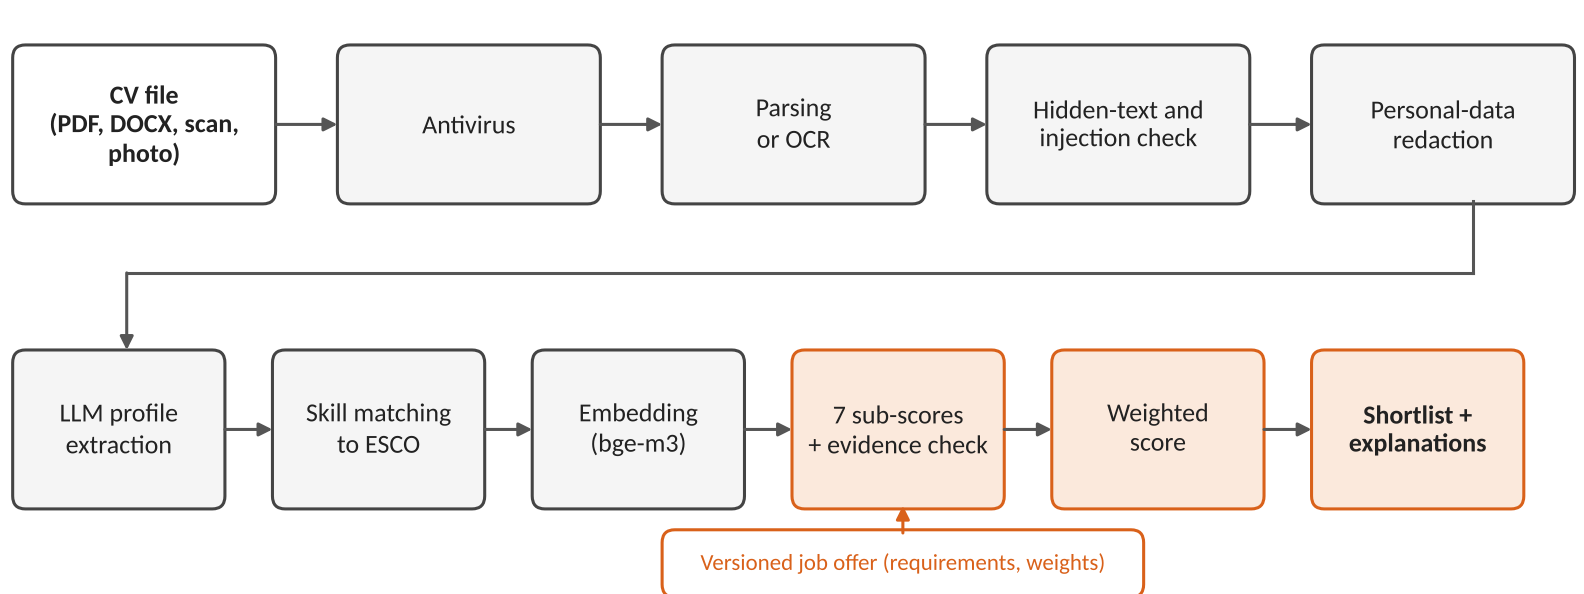
\includegraphics[width=\linewidth]{figures/pipeline.png}
{\small\sffamily\itshape Figure 1. Processing of a CV, from file to explained shortlist.}
\end{figure}

\begin{spectable}{L{3.6cm}L{1.6cm}X}
\thd{Sub-score} & \thd{Default weight} & \thd{What it measures} \\\midrule
\tb Skills & \tb 0.30 & \tb Required skills count double; ESCO hierarchy (``PostgreSQL'' satisfies ``SQL'') \\
\tb Requirements & \tb 0.25 & \tb Each requirement judged satisfied, partial or absent, with a verified quotation \\
\tb Experience & \tb 0.15 & \tb Relevant years against required years; over-qualification never penalised \\
\tb Semantic & \tb 0.15 & \tb Embedding similarity, a safety net against vocabulary variations \\
\tb Education & \tb 0.05 & \tb Level against requirement \\
\tb Languages & \tb 0.05 & \tb CEFR level per required language \\
\tb Location & \tb 0.05 & \tb Low weight because location can correlate with origin \\
\end{spectable}
The displayed score is 100 times the weighted sum; no weight may exceed 0.6. Weights are defaults, adjustable by the recruiter and calibrated on human-annotated data at the sprint 4 decision gate, and only kept if the gain is at least 0.02 nDCG and the bias tests remain compliant. A quotation is accepted only if it matches the CV text (fuzzy similarity of at least 90, at least 15 characters); otherwise the requirement is marked ``absent (not demonstrated)''. Explanations are generated from templates over structured data, never as free LLM text.

% ================= VI =================
\section{Functional requirements}
The platform has 58 functions in six areas. Priorities follow MoSCoW: \textbf{Must} (without it the platform does not work, is unsafe or illegal), Should (important, simplifiable; no Must depends on it), \textit{Could} (included if time allows, behind a feature flag). The cut line is explicit: no Must is ever postponed.

\Needspace{7\baselineskip}\subsection{Platform --- PLT}
\begin{spectable}{L{1.7cm}X L{1.4cm}}
\thd{ID} & \thd{Requirement} & \thd{Priority} \\\midrule
\tb PLT-01 & \tb Authentication and accounts & \tb \must \\
\tb PLT-02 & \tb Role-based access and multi-tenant organisations & \tb \must \\
\tb PLT-04 & \tb Transactional e-mail notifications & \tb \must \\
\tb PLT-06 & \tb Rate limiting, anti-abuse, antivirus on every file & \tb \must \\
\tb PLT-07 & \tb Observability: logs, metrics, alerts, error tracking & \tb \must \\
\tb PLT-08 & \tb Backups and tested restoration & \tb \must \\
\tb PLT-09 & \tb CI/CD and environments & \tb \must \\
\tb PLT-10 & \tb User documentation and in-product help & \tb \must \\
\tb PLT-03 & \tb Interface in French, English, Arabic (right-to-left) & \tb \should \\
\tb PLT-05 & \tb Two-factor authentication (TOTP) & \tb \should \\
\end{spectable}

\Needspace{7\baselineskip}\subsection{Employers and jobs --- ENT, JOB}
\begin{spectable}{L{1.7cm}X L{1.4cm}}
\thd{ID} & \thd{Requirement} & \thd{Priority} \\\midrule
\tb ENT-01 & \tb Company registration and organisation profile & \tb \must \\
\tb JOB-01 & \tb Structured job form and job lifecycle & \tb \must \\
\tb JOB-02 & \tb Job creation by chatbot (structured output, locked fields) & \tb \must \\
\tb JOB-03 & \tb Import by pasted text or file & \tb \must \\
\tb JOB-05 & \tb Public job page (SEO, JSON-LD structured data) & \tb \must \\
\tb JOB-04 & \tb Voice dictation & \tb \should \\
\tb JOB-06 & \tb Quality and bias check of the job post & \tb \should \\
\tb JOB-07, 08 & \tb Job templates and duplication; generated screening questions & \tb \could \\
\end{spectable}

\Needspace{7\baselineskip}\subsection{Intelligent ATS --- ATS}
\begin{spectable}{L{1.7cm}X L{1.4cm}}
\thd{ID} & \thd{Requirement} & \thd{Priority} \\\midrule
\tb ATS-01 & \tb Application without an account (magic link) & \tb \must \\
\tb ATS-02 & \tb Multi-format ingestion and parsing with OCR (PDF, DOCX, ODT, RTF, TXT, images, scans) & \tb \must \\
\tb ATS-03 & \tb Structured extraction and ESCO skill normalisation & \tb \must \\
\tb ATS-04 & \tb Hybrid score and ranking & \tb \must \\
\tb ATS-05 & \tb Configurable shortlist (top-N, threshold) & \tb \must \\
\tb ATS-06 & \tb Explanation per candidate, with evidence & \tb \must \\
\tb ATS-09 & \tb Application pipeline and human decision & \tb \must \\
\tb ATS-12 & \tb Defence against prompt injection and hidden text & \tb \must \\
\tb ATS-07, 08 & \tb Adjustable weights; counterfactuals and skill gaps & \tb \should \\
\tb ATS-10, 11 & \tb Human correction and feedback loop; anonymised blind view & \tb \should \\
\tb ATS-13, 14 & \tb Keyword-stuffing and inconsistency detection; duplicate detection & \tb \should \\
\tb ATS-15, 16 & \tb Candidate comparison; interview guide per candidate & \tb \could \\
\end{spectable}

\Needspace{7\baselineskip}\subsection{Candidates and matching --- CAN, MAT}
\begin{spectable}{L{1.7cm}X L{1.4cm}}
\thd{ID} & \thd{Requirement} & \thd{Priority} \\\midrule
\tb CAN-01 & \tb Candidate account and profile built from the CV & \tb \must \\
\tb CAN-02 & \tb Job search and browsing & \tb \must \\
\tb CAN-03 & \tb One-click application & \tb \must \\
\tb CAN-04 & \tb Application tracking with simplified status & \tb \must \\
\tb MAT-01 & \tb Job recommendations (``For you'' feed sorted by relevance, all jobs one click away) & \tb \must \\
\tb CAN-05 & \tb Job alerts & \tb \should \\
\tb MAT-02, 03 & \tb Talent suggestions to employers (opt-in); talent pool reuse across jobs & \tb \should \\
\tb CAN-06, 07 & \tb CV improvement tips; conversational candidate assistant & \tb \could \\
\end{spectable}

\Needspace{7\baselineskip}\subsection{Analytics, administration and GDPR --- ANA, ADM, RGPD}
\begin{spectable}{L{1.7cm}X L{1.4cm}}
\thd{ID} & \thd{Requirement} & \thd{Priority} \\\midrule
\tb ANA-01 & \tb Analytics dashboard per job & \tb \must \\
\tb ADM-01 & \tb Administration back-office & \tb \must \\
\tb ADM-03 & \tb Audit log & \tb \must \\
\tb RGPD-01 & \tb Consents and information to data subjects & \tb \must \\
\tb RGPD-02 & \tb Exercise of rights: access, erasure, human review & \tb \must \\
\tb RGPD-03 & \tb Automatic retention and purge & \tb \must \\
\tb ANA-02 & \tb Organisation dashboard & \tb \should \\
\tb ADM-02 & \tb AI supervision: models, costs, drift & \tb \should \\
\tb ANA-03 & \tb CSV export and PDF report & \tb \could \\
\end{spectable}

\Needspace{7\baselineskip}\subsection{Data and evaluation --- DAT}
\begin{spectable}{L{1.7cm}X L{1.4cm}}
\thd{ID} & \thd{Requirement} & \thd{Priority} \\\midrule
\tb DAT-01 & \tb Synthetic data generator & \tb \must \\
\tb DAT-02 & \tb Seed scripts (30-job production base, demo) & \tb \must \\
\tb DAT-03 & \tb Annotation tool for the reference dataset & \tb \must \\
\tb DAT-04 & \tb Automated AI evaluation bench & \tb \must \\
\end{spectable}

\Needspace{7\baselineskip}\subsection{Effort and capacity}
\begin{spectable}{L{6cm}L{2cm}L{2.2cm}X}
\thd{Priority} & \thd{Functions} & \thd{Person-days} & \thd{Share of 190} \\\midrule
\tb Must (functions) & \tb 36 & \tb 106 & \tb 56\,\% \\
\tb Must (cross-cutting work: annotation, load test, security review, release) & \tb --- & \tb 10 & \tb 5\,\% \\
\tb Should & \tb 15 & \tb 33.5 & \tb 18\,\% \\
\tb Could & \tb 7 & \tb 14.5 & \tb 8\,\% \\
\tb Reserve for contingencies & \tb --- & \tb 26 & \tb 14\,\% \\
\end{spectable}
Capacity is 3 people $\times$ 16 weeks $\times$ 5 days = 240 person-days, minus the final report (20), the defence (6) and meetings and learning (24), leaving \textbf{190 productive person-days}. The Must load is 116 person-days, 61\,\% of capacity.

% ================= VII =================
\section{Data protection and AI regulation}
\Needspace{7\baselineskip}\subsection{Roles}
The recruiting company is the \textbf{data controller} of its applications; the platform is its \textbf{processor} (Article 28 contract in the employer terms) and is controller for candidate accounts, matching and security. For the EU AI Act, the team is the \textbf{provider} of the system and each recruiting company is a \textbf{deployer}.

\Needspace{7\baselineskip}\subsection{Lawful basis and principles}
\begin{spectable}{L{5cm}X}
\thd{Processing} & \thd{Basis or measure} \\\midrule
\tb Application & \tb Pre-contractual measures (Art.\,6.1.b) \\
\tb Talent pool, visibility, alerts & \tb Consent (Art.\,6.1.a), versioned and time-stamped \\
\tb Security and audit & \tb Legitimate interest (Art.\,6.1.f) \\
\tb Automated decisions & \tb None: no decision based solely on automated processing; information on the logic; right to human intervention and to contest \\
\tb Minimisation & \tb No photo, birth date or nationality requested; sensitive attributes excluded from matching; audio deleted after transcription \\
\end{spectable}
A Data Protection Impact Assessment (DPIA) is performed at sprint 2 using the CNIL tool and updated before launch. A processing register is kept in the repository.

\Needspace{7\baselineskip}\subsection{Retention, deletion and breaches}
Full erasure (database, files, embeddings, caches) is completed within 30 days and verified by test; backups are purged within 35 days. A personal-data breach follows the 72-hour notification procedure of the runbook.

\Needspace{7\baselineskip}\subsection{Sub-processors}
Mistral AI, Hetzner, Backblaze and Brevo (EU); Sentry, Grafana Cloud and Langfuse (EU region); Cloudflare (Turnstile captcha). Each has a recorded data processing agreement, and ``no retention / no training'' options are enabled where available.

\Needspace{7\baselineskip}\subsection{EU AI Act}
Recruitment and candidate evaluation are \textbf{high-risk} systems (Annex III, point 4.a). Following Regulation (EU) 2026/1744, these obligations apply from 2 December 2027; prohibited practices (Article 5) already apply. The project applies the requirements now.
\begin{spectable}{L{4.2cm}X}
\thd{Requirement} & \thd{How it is covered} \\\midrule
\tb Risk management (Art.\,9) & \tb Risk register, Section XII \\
\tb Data governance (Art.\,10) & \tb Four evaluation datasets, FR/EN/AR representativeness measured \\
\tb Technical documentation (Art.\,11) & \tb This specification and a public model card \\
\tb Logging (Art.\,12) & \tb Append-only chained audit log \\
\tb Transparency (Art.\,13) & \tb ``How the AI works'' page, user documentation \\
\tb Human oversight (Art.\,14) & \tb Pipeline, explanations, no automatic rejection, measurement of automation bias \\
\tb Accuracy and robustness (Art.\,15) & \tb Evaluation bench, injection defence \\
\end{spectable}
Formal quality management, conformity assessment and EU database registration are outside the project and listed as prerequisites for real commercialisation.

\Needspace{7\baselineskip}\subsection{Fairness measures}
Known bias sources are weaker extraction for Arabic or scanned CVs, the weight of prestigious schools, location, career gaps and name bias in the LLM. Measures: metrics broken down by language and format; ``to check'' lane instead of down-ranking; names removed before evaluation; no penalty for career gaps; bounded weights; counterfactual tests; anonymised view. Demographic data is deliberately not collected, so fairness is verified on synthetic pairs only; this limit is stated in the model card.

% ================= VIII =================
\section{Non-functional requirements}
Every requirement is measurable and traced to the production-readiness criteria (Section XIV) and to a test.
\begin{spectable}{L{2.6cm}X L{4.4cm}}
\thd{Area} & \thd{Requirement} & \thd{Target} \\\midrule
\tb Performance & \tb Public job page; authenticated API reads & \tb p95 $\le$ 500 ms; p95 $\le$ 300 ms \\
\tb & \tb Application upload (synchronous part) & \tb p95 $\le$ 1 s \\
\tb & \tb CV uploaded to score available & \tb p95 $\le$ 90 s \\
\tb & \tb Burst ingestion; shortlist recalculation & \tb 1,000 CVs in 60 min; $\le$ 5 s \\
\tb Capacity & \tb Verified by load test on synthetic data & \tb 500 active jobs, 10,000 profiles, 20,000 applications, 200 concurrent visitors \\
\tb Security & \tb TLS 1.2+, HSTS, strict CSP; OWASP ASVS level 2 & \tb Tested; 0 high ZAP alert \\
\tb & \tb Organisation isolation; secrets; file handling & \tb 100\,\% of routes; SOPS + age; 10 MB, antivirus, signed URLs of 5 min \\
\tb & \tb Rate limits & \tb e.g.\ 5 applications/h/IP, 300 API calls/min/user \\
\tb Availability & \tb Monthly availability; recovery point; recovery time & \tb $\ge$ 99.5\,\%; $\le$ 15 min; $\le$ 4 h \\
\tb & \tb AI provider outage & \tb Degraded mode, queues, local OCR fallback \\
\tb Accessibility & \tb WCAG 2.1 AA; responsive from 360 px; FR/EN/AR with RTL & \tb 0 critical violation \\
\tb Observability & \tb Centralised logs 30 days; error tracking; 8 alerts & \tb Each alert fired once in staging \\
\tb AI quality & \tb Explanation for every scored application; reproducibility & \tb 100\,\%; score deviation $\le$ 0.01; 4/5 rule $\ge$ 0.8 \\
\tb Software quality & \tb Full CI; strict typing; test coverage & \tb $\ge$ 70\,\% overall, $\ge$ 80\,\% on core modules \\
\tb Operations & \tb Zero-downtime deployment; rollback & \tb $\le$ 10 min \\
\end{spectable}

% ================= IX =================
\section{Architecture}
\Needspace{7\baselineskip}\subsection{Overview}
A \textbf{modular monolith} (one Python code base, one deployment), a Next.js frontend and a single separate process, the \textbf{worker}, built from the same image as the API. The worker exists for four measurable reasons: parsing and AI take 5 to 60 s per CV, which is incompatible with an HTTP request; the embedding model and antivirus use about 4 GB of memory that should not be duplicated in every API process; retries and priority queues (interactive chatbot before scoring before alerts); and independent scaling. No other service is created.

\begin{figure}[h]
\centering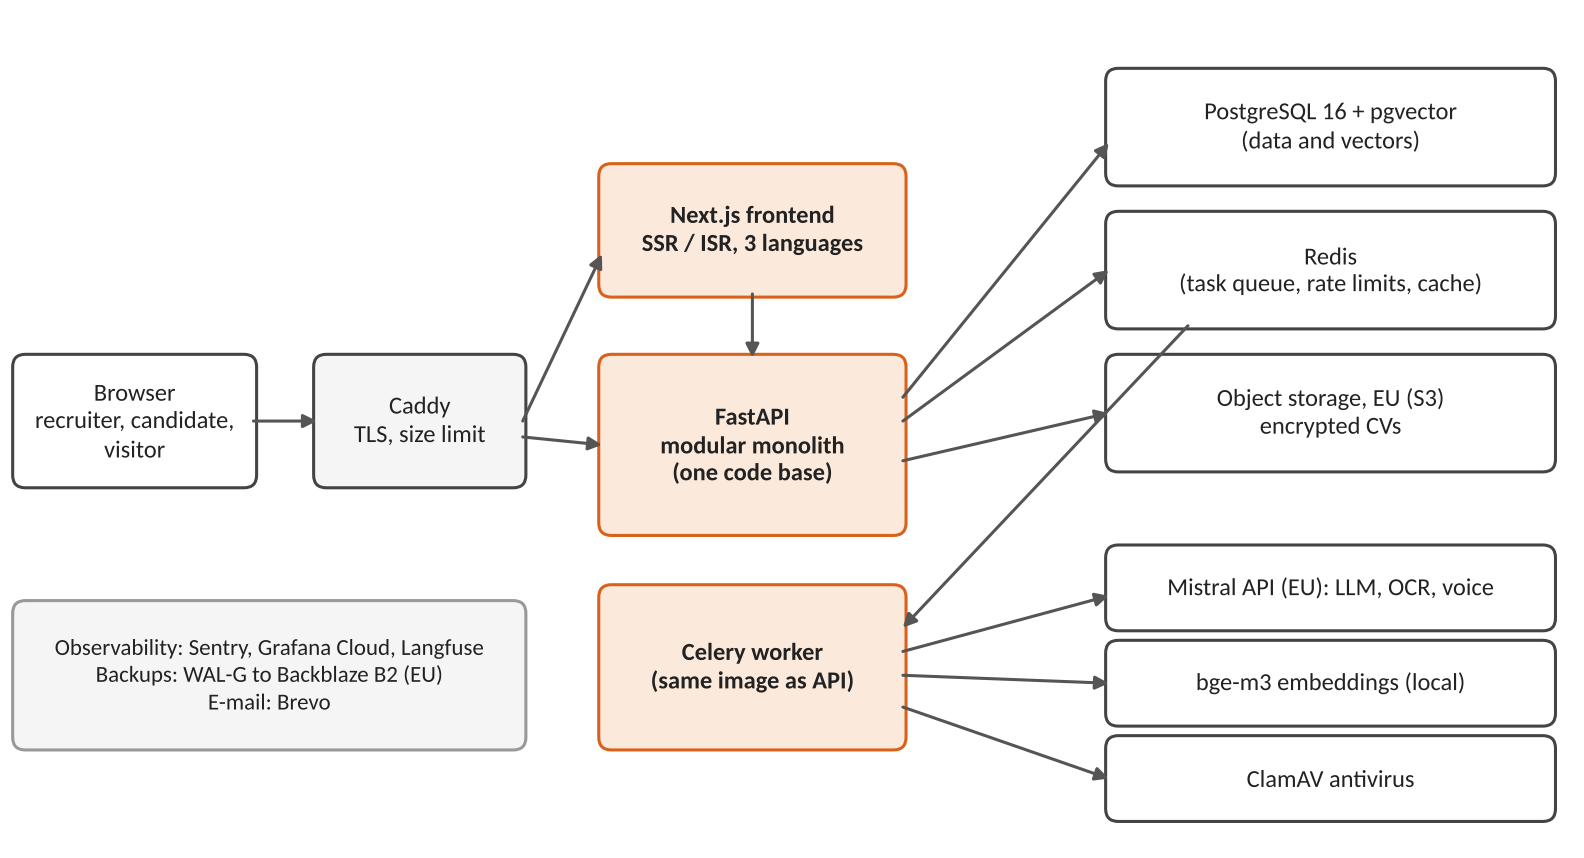
\includegraphics[width=\linewidth]{figures/architecture.png}
{\small\sffamily\itshape Figure 2. Runtime architecture on a single European virtual machine.}
\end{figure}

\Needspace{7\baselineskip}\subsection{Technology choices}
\begin{spectable}{L{2.5cm}L{5cm}X}
\thd{Layer} & \thd{Choice} & \thd{Reason} \\\midrule
\tb Frontend & \tb Next.js 15, TypeScript, Tailwind CSS, shadcn/ui & \tb Server rendering for SEO; accessible components; RTL support \\
\tb Backend & \tb Python 3.12, FastAPI, Pydantic v2, SQLAlchemy 2 & \tb Python AI ecosystem; schemas shared with LLM outputs \\
\tb Database & \tb PostgreSQL 16 + pgvector (HNSW) & \tb One system for data, vectors, transactions and backup; fewer than 1 million vectors \\
\tb Background tasks & \tb Celery 5 + Redis 7 & \tb Mature retries, priorities, scheduling \\
\tb LLM & \tb Mistral Small via EU API, JSON-constrained output & \tb EU hosting, low cost, open weights, good FR/AR; confirmed at sprint 4 against an alternative \\
\tb Embeddings & \tb BAAI bge-m3 (1,024 dimensions), run locally & \tb Multilingual including Arabic, free, deterministic, no data sent out \\
\tb Parsing and OCR & \tb PyMuPDF4LLM, docx2python; Mistral OCR with Tesseract fallback & \tb Light and fast; Arabic quality; local fallback for resilience \\
\tb Skill taxonomy & \tb ESCO v1.2 (FR/EN) + local extension of about 600 tech skills & \tb European, open, stable identifiers \\
\tb Hosting & \tb Hetzner Cloud VM (8 vCPU, 16 GB), Docker Compose, Caddy & \tb Cost/performance, EU, automatic HTTPS; Kubernetes judged oversized \\
\tb Delivery & \tb GitHub Actions, GHCR, SOPS + age & \tb Free minutes suffice; secrets encrypted in Git \\
\end{spectable}
The LLM client is behind an interface (\texttt{complete\_json(schema, messages)}) so the provider can be changed without touching business modules. Model versions and prices are rechecked at sprint 1.

\Needspace{7\baselineskip}\subsection{AI safeguards}
\begin{spectable}{L{4cm}X}
\thd{Risk} & \thd{Safeguard} \\\midrule
\tb Injection in a CV or job post & \tb Hidden text removed, delimiters, output under schema, score computed outside the LLM, detector, adversarial tests \\
\tb Hallucination & \tb Entity grounding in the text, evidence verification, ``null rather than invent'' \\
\tb Bias & \tb Sensitive attributes removed, no over-qualification penalty, counterfactual tests in CI \\
\tb Non-determinism & \tb Temperature 0, cache by fingerprint, pinned versions, re-run test \\
\tb Provider outage & \tb Three exponential retries, degraded mode, Tesseract fallback \\
\tb Cost & \tb Ceilings per organisation, alerts, cache \\
\tb Data leakage & \tb Pseudonymisation, contract without retention or training, EU hosting \\
\end{spectable}

\Needspace{7\baselineskip}\subsection{Deployment pipeline}
Pull request: lint, typing, unit and integration tests, secret scan, regression evaluation when AI code changes. Merge to main: image build, vulnerability scan, deployment to staging, end-to-end and accessibility tests. Production: manual approval, pre-deployment backup, migration, switch with a 2-minute health check and automatic rollback. Nightly: full evaluation, dependency updates; weekly: ZAP scan.

% ================= X =================
\section{Integrations}
\begin{spectable}{L{3.6cm}L{5.4cm}X}
\thd{Service} & \thd{Use} & \thd{Location / notes} \\\midrule
\tb Mistral AI & \tb LLM, OCR, voice transcription & \tb EU; no retention or training \\
\tb Hetzner & \tb VM, staging, object storage for CVs & \tb EU \\
\tb Backblaze B2 & \tb Encrypted off-site backups (WAL-G) & \tb EU region \\
\tb Brevo & \tb Transactional e-mail & \tb EU; free quota suffices at launch \\
\tb Cloudflare Turnstile & \tb Captcha on public forms & \tb Free, no ad tracking \\
\tb Sentry, Grafana Cloud, Langfuse & \tb Errors, metrics and logs, LLM traces & \tb EU region \\
\tb GitHub & \tb Repository, CI/CD, container registry & \tb --- \\
\end{spectable}

% ================= XI =================
\section{KPIs}
\Needspace{7\baselineskip}\subsection{Principle}
AI targets are measured \textbf{only on a human-annotated dataset}: 10 real jobs $\times$ 50 CVs (30 real, consented, plus 20 realistic CVs written by people), annotated by two annotators, one of them a professional recruiter. They are working hypotheses with a 95\,\% bootstrap confidence interval. The primary success criterion is relative: \textbf{beat the keyword baseline (BM25)}. A missed target that is honestly measured does not invalidate acceptance; a missing measurement does.

\Needspace{7\baselineskip}\subsection{Target set}
\begin{spectable}{L{1cm}X L{4.2cm}}
\thd{ID} & \thd{KPI} & \thd{Target} \\\midrule
\tb K1 & \tb Skill extraction F1 (after normalisation) & \tb $\ge$ 0.80 \\
\tb K2 & \tb Contact fields accuracy (e-mail, phone) & \tb $\ge$ 0.95 \\
\tb K3 & \tb Ranking quality, nDCG@10 & \tb $\ge$ 0.75 and BM25 + 0.05 \\
\tb K4 & \tb Precision@N (relevance $\ge$ 2), N = 10 & \tb $\ge$ 0.70 \\
\tb K5 & \tb System/recruiter agreement (weighted kappa) & \tb Human-human kappa $-$ 0.10 \\
\tb K6 & \tb Score gap on counterfactual pairs (name, gender, origin) & \tb Mean $<$ 0.01; max $<$ 0.03 \\
\tb K7 & \tb CV uploaded to score available & \tb p95 $\le$ 90 s \\
\tb K8 & \tb Time to create a full job with the chatbot & \tb Median $\le$ 5 min \\
\tb K9 & \tb Monthly availability of public pages and API & \tb $\ge$ 99.5\,\% \\
\tb K10 & \tb Perceived usefulness of explanations & \tb SUS $\ge$ 70; $\ge$ 80\,\% judged useful \\
\tb K11 & \tb Production base & \tb 30 active jobs from 10 companies, 100\,\% of journeys validated \\
\end{spectable}

\Needspace{7\baselineskip}\subsection{Evaluation datasets}
\begin{spectable}{L{3cm}L{4.8cm}X}
\thd{Dataset} & \thd{Content} & \thd{Use} \\\midrule
\tb SYNTH-REG & \tb 300 CVs, 20 jobs, planted relevance & \tb CI non-regression \\
\tb SYNTH-LOAD & \tb 10,000+ profiles, 500 jobs, 20,000 applications & \tb Load test \\
\tb SYNTH-ADV / BIAS & \tb 40 trap CVs; 200 counterfactual pairs & \tb Robustness and fairness \\
\tb G-REAL (DEV / TEST) & \tb 50 CVs, 10 real jobs, 500 annotated pairs & \tb Calibration (5 jobs), final measure (5 jobs) \\
\end{spectable}
Synthetic data serves volume, load, regression, adversarial and bias tests only; any claim about real performance rests solely on G-REAL. The limits of synthetic data are written into the evaluation report.

% ================= XII =================
\section{Costs and risks}
\Needspace{7\baselineskip}\subsection{Running costs}
\begin{spectable}{L{7cm}X}
\thd{Item} & \thd{EUR / month} \\\midrule
\tb Production VM (8 vCPU, 16 GB) & \tb $\approx$ 30 \\
\tb Staging VM (4 vCPU, 8 GB) & \tb $\approx$ 15 \\
\tb Object storage for CVs & \tb $\approx$ 5 \\
\tb Off-site backups; domain name & \tb $\approx$ 1 + 1 \\
\tb AI at base load (about 1,500 applications and 60 jobs per month) & \tb $\approx$ 4 \\
\tb E-mail, monitoring, captcha, CI (free tiers) & \tb 0 \\
\tb \textbf{Total at base load} & \tb \textbf{$\approx$ 56, rounded to 60} \\
\end{spectable}
AI cost is about 0.002~\texteuro{} per application and about 0.01~\texteuro{} per job created by chatbot. At the capacity target (20,000 applications a month) AI adds about 40~\texteuro{} a month. The project total over four months is \textbf{about 330~\texteuro{}}: operation 225, synthetic data generation 40, evaluation and load test 10, 20\,\% reserve 55. Provider budgets are capped (alert at 50\,\%, cut-off at 100\,\% of 30~\texteuro{} a month).

\Needspace{7\baselineskip}\subsection{Main risks}
\begin{spectable}{L{4.2cm}X}
\thd{Risk} & \thd{Mitigation and fallback} \\\midrule
\tb Delay on Must functions & \tb 61\,\% Must load, 26-day reserve, cut line at week 12; if velocity falls below 80\,\%, replan and cut Should \\
\tb Fewer than 10 companies or 20 real candidates & \tb Outreach from sprint 1 through the school; fall back to school and partner internship offers \\
\tb Weak Arabic extraction & \tb Metrics per language, ``to check'' lane, systematic human review of Arabic CVs if F1 $<$ 0.70 \\
\tb Ranking not better than BM25 & \tb Baselines from sprint 4, decision gate, error analysis and prompt adjustment \\
\tb AI provider price or version change & \tb Provider abstraction, pinned versions, ceilings, alternative provider \\
\tb Security incident & \tb Dedicated review, ZAP scan, 72-hour breach procedure \\
\tb Low availability of the HR referent & \tb Sessions planned from sprint 1; second recruiter from the school network \\
\tb Recruiter over-trust (automation bias) & \tb Reasons displayed before grouped rejection, open-rate measured; batch limited to 50 if open rate $<$ 20\,\% \\
\tb Fraudulent job posts & \tb Organisation verification, moderation, reporting, immediate suspension \\
\tb Loss of a team member & \tb Cross review, documentation, shared ownership; switch to a 2-person plan (Must only) \\
\end{spectable}

% ================= XIII =================
\section{Delivery phases}
\Needspace{7\baselineskip}\subsection{Principle}
There is \textbf{one} production release, Release 1.0, opened publicly at the end of week 14. A working skeleton (HTTPS, authentication, CI/CD, backups, error tracking) is deployed to production from sprint 1 behind a ``coming soon'' page, so that operations are de-risked early.

\Needspace{7\baselineskip}\subsection{Sprints}
\begin{spectable}{L{0.9cm}L{1.5cm}X L{3.6cm}}
\thd{Sprint} & \thd{Weeks} & \thd{Content} & \thd{Milestone} \\\midrule
\tb S1 & \tb 1--2 & \tb Scoping, mock-ups, production skeleton, annotation guide & \tb Skeleton live over HTTPS \\
\tb S2 & \tb 3--4 & \tb Accounts, organisations, job form, import, public page, application without account, DPIA & \tb First public job and application \\
\tb S3 & \tb 5--6 & \tb Parsing and OCR, extraction, ESCO, injection defence, synthetic generator, annotation & \tb Reference dataset frozen \\
\tb S4 & \tb 7--8 & \tb Score, shortlist, explanations, evaluation bench, calibration & \tb AI decision gate: LLM, embeddings, weights \\
\tb S5 & \tb 9--10 & \tb Chatbot, candidate accounts, one-click apply, recommendations, pipeline & \tb Complete candidate journey \\
\tb S6 & \tb 11--12 & \tb Analytics, back-office, GDPR, audit, security review & \tb Cut line: 100\,\% of Must done \\
\tb S7 & \tb 13--14 & \tb Should functions, load and bias tests, acceptance, onboarding of 10 companies & \tb \textbf{Public opening of Release 1.0} \\
\tb S8 & \tb 15--16 & \tb Fixes, Could functions if margin, report, defence & \tb Code freeze week 15; defence \\
\end{spectable}

\Needspace{7\baselineskip}\subsection{Cut-line rule}
If a Must is unfinished at the end of sprint 6, every Should and Could is frozen until it is done; Should functions are then taken by value order. Any Should or Could not finished by week 15 is switched off by feature flag and is not part of the release. With a team of two (about 125 person-days) only Must functions are possible; with four (about 255), all Could functions fit.

% ================= XIV =================
\section{Acceptance, testing and handover}
\Needspace{7\baselineskip}\subsection{Definition of production-ready}
Release 1.0 is production-ready if and only if the following 16 criteria are proven at acceptance, each tied to an evidence and an automated or documented test.
\begin{spectable}{L{0.9cm}L{4.4cm}X}
\thd{ID} & \thd{Criterion} & \thd{Evidence required} \\\midrule
\tb 1 & \tb Public HTTPS deployment & \tb SSL Labs grade A or better; HSTS; redirect \\
\tb 2 & \tb Authentication and RBAC & \tb Role-by-endpoint matrix 100\,\%; isolation tests green \\
\tb 3 & \tb Secret management & \tb No secret in Git history; rotation tested once \\
\tb 4 & \tb Automatic backups & \tb Daily full + continuous WAL, off-site, encrypted; RPO $\le$ 15 min \\
\tb 5 & \tb Tested restoration & \tb Monthly automated restore; timed manual exercise; RTO $\le$ 4 h \\
\tb 6 & \tb CI/CD with automated tests & \tb Lint, typing, tests, E2E, image scan, AI regression; deploy only from main after approval \\
\tb 7 & \tb Monitoring and alerting & \tb Dashboards; 8 alerts each fired once in staging \\
\tb 8 & \tb Central logs and error tracking & \tb 30-day JSON logs; errors tagged by release \\
\tb 9 & \tb Rate limiting and anti-abuse & \tb 429 responses verified; captcha; antivirus on all files \\
\tb 10 & \tb GDPR consent & \tb Notices published; versioned time-stamped consents \\
\tb 11 & \tb Data deletion & \tb Complete erasure within 30 days; backups purged within 35 days \\
\tb 12 & \tb Audit log & \tb 18 sensitive event types logged, append-only, admin-readable \\
\tb 13 & \tb Runbook & \tb 10 procedures, each run once by someone who did not write it \\
\tb 14 & \tb User documentation & \tb Recruiter, candidate and admin guides; FAQ; ``How the AI works'' page \\
\tb 15 & \tb Load test result & \tb k6 report at the capacity target; SLOs met \\
\tb 16 & \tb Production base & \tb 30 jobs from 10 companies; 20 to 30 real applications end to end \\
\end{spectable}

\Needspace{7\baselineskip}\subsection{Global acceptance criteria (week 14)}
\begin{enumerate}
  \item 16 of 16 production-readiness criteria proven, checklist signed by the supervisor.
  \item At least 10 real companies have published at least 3 jobs each, with public page, application flows, parsing, score, shortlist of chosen size N, explanations for all candidates and analytics.
  \item 20 to 30 real applications processed end to end without technical help, including at least 3 scanned or photographed CVs and 3 in Arabic or bilingual.
  \item 36 of 36 Must functions delivered and tested, with traceability from function to acceptance criterion to test.
  \item K1 to K6 measured and published with confidence intervals; K3 above BM25 reached, or the gap documented with error analysis.
  \item No rejection without a human in the audit over the whole period; DPIA validated; erasure and human-review requests tested.
  \item No open blocking defect; at most 5 major defects with a documented workaround.
  \item SUS $\ge$ 70 with 5 recruiters and 5 candidates; K8 measured.
\end{enumerate}

\Needspace{7\baselineskip}\subsection{Testing strategy}
Test pyramid with unit, integration and end-to-end tests (Playwright and axe-core on staging); AI tests (extraction, scoring reproducibility, shortlist edge cases with N in $\{1,5,10,37,200\}$); bias tests on counterfactual pairs in CI; security tests (isolation on every route, OWASP ZAP, secret and image scans); GDPR tests (erasure, consents); load tests with k6 on synthetic data; usability tests with real users. Coverage is at least 70\,\% overall and 80\,\% on scoring, shortlist, authentication and GDPR modules.

\Needspace{7\baselineskip}\subsection{Deliverables}
\begin{spectable}{L{1cm}X L{2.4cm}}
\thd{ID} & \thd{Deliverable} & \thd{Due} \\\midrule
\tb L-01 & \tb Approved specification & \tb Week 1 \\
\tb L-02 & \tb Figma mock-ups, 32 screens, desktop and mobile & \tb Complete week 10 \\
\tb L-03 & \tb Source code, README, architecture decision records & \tb Continuous \\
\tb L-04 & \tb Release 1.0 in production on a public URL & \tb End of week 14 \\
\tb L-05 & \tb Versioned datasets and generation and evaluation tools & \tb Week 13 \\
\tb L-06 & \tb AI evaluation report and public model card & \tb Week 14 \\
\tb L-07 & \tb Load test report & \tb Week 14 \\
\tb L-08 & \tb Compliance file: DPIA, register, notices, AI Act mapping & \tb Week 14 \\
\tb L-09 & \tb Runbook and operations documentation & \tb Week 14 \\
\tb L-10 & \tb User documentation (recruiter, candidate, admin) & \tb Week 14 \\
\tb L-11 & \tb Final report, defence slides, 5-minute demo video & \tb Week 16 \\
\end{spectable}

\Needspace{7\baselineskip}\subsection{Runbook}
Ten mandatory procedures: site down; full restoration on a new VM; point-in-time restoration; LLM or OCR provider outage; saturated worker queue; full disk; rotation of a compromised secret; data breach (72-hour notification); rollback of a deployment or migration; fraudulent job post or mass abuse.

% ================= XV =================
\section{Team and responsibilities}
\begin{spectable}{L{1.2cm}L{3.8cm}X}
\thd{} & \thd{Main role} & \thd{Responsibilities and secondary role} \\\midrule
\tb M1 & \tb AI lead & \tb Parsing, extraction, ESCO, score, explanations, evaluation, synthetic data. Writes the model card; does not annotate, to keep the reference set independent \\
\tb M2 & \tb Backend and DevOps lead & \tb Architecture, API, worker, security, CI/CD, deployment, observability, technical GDPR. Technical product owner \\
\tb M3 & \tb Frontend and product lead & \tb Next.js, UX, accessibility, i18n, chatbot interface, E2E tests, documentation. Annotator and scrum master \\
\end{spectable}
Rituals: planning and review every two weeks with the supervisor and the HR referent; 15-minute daily meeting; mandatory cross code review. The specification is explicit enough for another engineer to continue the work without redesigning the system, and the runbook and architecture decision records support future continuity.

% ================= XVI =================
\section{Decisions to validate}
Five decisions condition the start of development.
\begin{spectable}{L{1cm}L{4cm}X}
\thd{ID} & \thd{Decision} & \thd{Content} \\\midrule
\tb D1 & \tb Human decides & \tb The AI sorts, ranks and explains; no rejection is sent without a traced human action (grouped rejection allowed after reading the reasons). It conditions GDPR and AI Act legality \\
\tb D2 & \tb Stack and hosting & \tb FastAPI, Next.js, PostgreSQL with pgvector, one Hetzner VM in the EU, Mistral (EU) as main AI provider, with a decision gate at sprint 4 \\
\tb D3 & \tb Transparent score & \tb Seven additive sub-scores with default weights 0.30 / 0.25 / 0.15 / 0.15 / 0.05 / 0.05 / 0.05; the LLM judges facts with verified evidence instead of giving a global score \\
\tb D4 & \tb Must scope & \tb 36 functions for 116 of 190 person-days, including chatbot, multilingual OCR, candidate recommendations and the synthetic generator; translated UI, voice dictation and talent suggestions are Should \\
\tb D5 & \tb Evaluation protocol & \tb 10 real jobs $\times$ 50 CVs, two annotators including a professional recruiter, main target ``beat BM25 by 0.05 nDCG@10''; requires finding the HR referent and volunteers from sprint 1 \\
\end{spectable}

% ================= ANNEX A =================
\Needspace{9\baselineskip}\section*{Annex A --- Vocabulary}
\addcontentsline{toc}{section}{\protect\numberline{}Annex A --- Vocabulary}
\begin{spectable}{L{3.4cm}X}
\thd{Term} & \thd{Definition} \\\midrule
\tb ATS & \tb Applicant Tracking System: software to manage applications \\
\tb Shortlist & \tb Subset of candidates proposed to the recruiter, of a size the recruiter chooses \\
\tb ESCO & \tb European taxonomy of skills, competences and occupations \\
\tb Embedding & \tb Numeric vector representing the meaning of a text, used to compare CVs and jobs \\
\tb LLM / OCR & \tb Large language model; optical character recognition for scanned documents \\
\tb BM25 & \tb Classic keyword-based ranking, used as the baseline to beat \\
\tb nDCG@10 & \tb Ranking quality measure over the top 10 results, between 0 and 1 \\
\tb MoSCoW & \tb Must, Should, Could, Won't prioritisation \\
\tb RPO / RTO & \tb Maximum tolerated data loss / maximum time to restore service \\
\tb SUS & \tb System Usability Scale; 70 is the usual threshold for acceptable usability \\
\tb DPIA & \tb Data Protection Impact Assessment (``AIPD'' in French) \\
\tb Counterfactual pair & \tb Two identical CVs differing only by name, gender or origin, used to detect bias \\
\tb Magic link & \tb Time-limited link giving an account-less candidate access to their application \\
\end{spectable}

% ================= ANNEX B =================
\Needspace{9\baselineskip}\section*{Annex B --- Review history of the specification}
\addcontentsline{toc}{section}{\protect\numberline{}Annex B --- Review history of the specification}
The full specification was approved at round 3 after 35 findings (3 blocking, 16 major, 16 minor), all fixed or refused with justification.
\begin{spectable}{L{2cm}L{3.4cm}L{1.6cm}L{1.4cm}L{1.4cm}X}
\thd{Round} & \thd{Version} & \thd{Blocking} & \thd{Major} & \thd{Minor} & \thd{Verdict} \\\midrule
\tb 1 & \tb Draft 1 (v1.0) & \tb 3 & \tb 12 & \tb 5 & \tb Rejected \\
\tb 2 & \tb Draft 2 (v1.1) & \tb 0 & \tb 4 & \tb 8 & \tb To revise \\
\tb 3 & \tb Draft 3 (v1.2, v1.3) & \tb 0 & \tb 0 & \tb 3 & \tb \textbf{Approved} \\
\end{spectable}
The three blocking findings of round 1 shaped the design: a Must load of 143 person-days against about 170 available was reduced to 116 of 190; the automatic rejection of non-shortlisted candidates was removed as contrary to GDPR Article 22 and AI Act Article 14; and circular evaluation, where synthetic labels came from the same function as the score, was replaced by planted relevance independent of the scorer and human-annotated real data. Major corrections include a configurable shortlist policy instead of a hard-coded top 10, a modular monolith instead of three microservices, PostgreSQL with pgvector instead of a dedicated vector database, prompt-injection defence, deterministic scoring, Arabic normalisation through multilingual embeddings, a measurable definition of production-ready, and a cost model.

\end{document}
